% Chapter 3

\chapter{Hyperledger Fabric} % Main chapter title

\label{Chapter3} % For referencing the chapter elsewhere, use \ref{Chapter1} 

\lhead{Capítulo 3. \emph{Hyperledger Fabric}} % This is for the header on each page - perhaps a shortened title
\setstretch{1.1} % Line spacing of 1.1
Para poder proceder con el diseño de un prototipo resulta necesario conocer los detalles de la implementación de la plataforma elegida. Por eso, el objetivo del presente capítulo es adquirir un profundo conocimiento de terminología, diseño y funcionamiento de Hyperledger Fabric.

%----------------------------------------------------------------------------------------
%	SECTION 1
%----------------------------------------------------------------------------------------

\section{Composición de la red Blockchain}
\label{composicion_red_blockchain}
%explicacion de peers y ledger
Como también en otras implementaciones ya estudiadas, la red se compone por un conjunto de nodos participantes o \textit{peers}, que intercambian mensajes sobre el estado del Blockchain. \textit{Peers} son los elementos más fundamentales de Hyperledger Fabric, ya que almacenan el \textit{ledger}, o el Blockchain.
Los términos \textit{ledger} o Blockchain este contexto describen el mismo concepto y se van a utilizar ambos términos de forma intercambiable, hasta aclarar la diferencia en la sección \ref{sec:ledger_and_world_state}.
%explicación de chaincode
Además, los \textit{peers} ejecutan los \textit{smart contracts}, que en Hyperldeger Fabric se llaman \textit{chaincodes}. Existen dos operaciones sobre el Blockchain: la de lectura y la de escritura. Ambas operaciones tienen que ser implementadas en el \textit
{chaincode}: la existencia de una instancia del \textit{ledger} solo no permite leer o modificar información.

Una colección de \textit{peers} cumple con las siguientes características:
\begin{itemize}
    \item Cada \textit{peer} que pertenece a la red, almacena una instancia del \textit{ledger} y una instancia del \textit{chaincode}.
    \item Al existir instancias iguales en todos los nodos, se evita un único punto de fallo: Cuando el \textit{ledger} es modificado, cada \textit{peer} actualiza su instancia.
    \item Ya que cada \textit{peer} es capaz que acceder y modificar el Blockchain, una aplicación que necesita leer o modificar el \textit{ledger}, lo tiene que hacer a través del \textit{peer}.
    \begin{figure}[H] % Example image
        \center{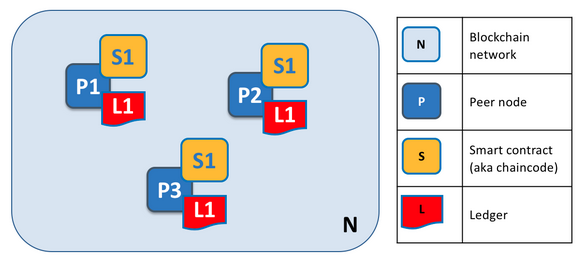
\includegraphics[width=1.0\linewidth]{Figures/Selection_169.png}}
        \caption{Una red Blockchain con 3 \textit{peers}: Cada \textit{peer} corre una instancia idéntica del \textit{chaincode} y del \textit{ledger}. De \cite{hlf-peers}.}
        \label{fig:Selection_169}
    \end{figure}  
    
\end{itemize}
La figura \ref{fig:Selection_169} ilustra lo descrito: En una red se encuentran 3 \textit{peers}, donde cada uno tiene una copia del \textit{ledger} y del \textit{chaincode}. \textit{Peers} pueden ser agregados o eliminados de la red de forma dinámica, según las necesidades de los administradores. No existen limitaciones con respecto a la cantidad de \textit{peers} que pueden conformar una red.

\section{La existencia de varios \textit{ledgers}}
En la sección anterior se explicó que cada \textit{peer} almacena su instancia del \textit{ledger} y del \textit{chaincode} y que los datos pueden ser actualizados solamente a través del \textit{chaincode}. Una analogía sería permitir la lectura y escritura de una base de datos relacional solamente a través de llamadas a una API, en vez de ejecutar instrucciones SQL directamente.

Una particularidad de Hyperledger Fabric consiste en posibilitar la existencia de varios \textit{ledgers}: Un \textit{peer} puede almacenar diferentes Blockchains como también diferentes \textit{chaincodes} que acceden al Blockchain correspondiente. La figura \ref{fig:Selection_170} visualiza la situación descrita: El \textit{peer} P1 aloja \textit{ledger} L1, al cual puede acceder con los \textit{chaincodes} S1 y S2. A su vez, aloja \textit{ledger} L2, accesible a través de S1 y S3.

\begin{figure}[H] % Example image
    \center{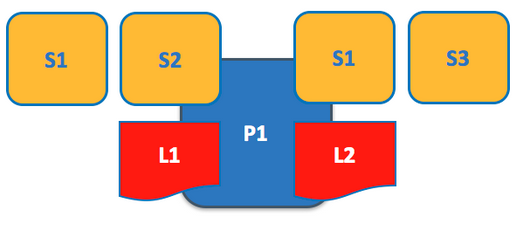
\includegraphics[width=0.7\linewidth]{Figures/Selection_170.png}}
    \caption{Un peer que aloja 2 \textit{ledgers} y 3 diferentes \textit{chaincodes}. De \cite{hlf-peers}.}
    \label{fig:Selection_170}
\end{figure}

No existen límites con respecto a esa arquitectura: un peer puede alojar tantos \textit{ledgers} y \textit{chaincodes} como se desea. Tampoco hay una relación requerida entre la cantidad de \textit{ledgers} y \textit{chaincode}: un peer teóricamente puede alojar un \textit{ledger} sin \textit{chaincode} que acceda a él. Cada \textit{ledger} almacena información independientemente de otros \textit{ledgers} y funciona como un Blockchain diferente.

En un ambiente de Blockchains privados, el paradigma descrito es de mucha utilidad: Un conjunto de empresas puede decidir compartir información en un \textit{ledger} al cual acceden todos los participantes, pero también pueden existir \textit{ledgers} entre un subconjunto de participantes, permitiendo un grado de privacidad mayor. En la figura \ref{fig:ledgers} se muestra el escenario descrito.

\begin{figure}[H] % Example image
    \center{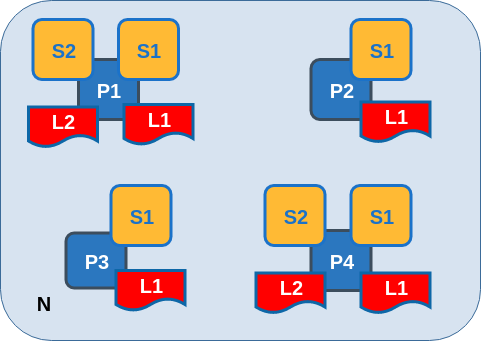
\includegraphics[width=0.7\linewidth]{Figures/ledgers.png}}
    \caption{Una red con 2 \textit{ledgers} diferentes: \textit{peers}  P2 y P3 no saben de la existencia del \textit{ledger} L2, sin embargo, todos los \textit{peers}  comparten información en el \textit{ledger} L1. }
    \label{fig:ledgers}
\end{figure}

Recordando las implementaciones analizadas en el capítulo \ref{Chapter2}, por cada red de participantes existía un sólo Blockchain que almacenaba todas las transacciones efectuadas de la red: La arquitectura de Hyperledger Fabric permite mantener una multitud de Blockchains en una misma red, donde los \textit{peers}  solamente tienen conocimiento de los \textit{ledgers}  que alojan.

\section{Aplicaciones y la red Blockchain}
\label{sec:aplicaciones_y_redBC}

Como se mencionó en la sección \ref{composicion_red_blockchain}, es necesario que aplicaciones accedan al Blockchain estableciendo una conexión con los \textit{peers}. Para lograr eso, Hyperledger Fabric provee SDKs en los lenguajes Java, Python, Go y Nodejs. Programadores pueden utilizar las funciones del SDK para conectarse a la API expuesta por cada \textit{peer} e invocar \textit{chaincode}.

Una aplicación se puede conectar a un \textit{peer} para consultar información existente en el Blockchain o para actualizar su estado. El flujo de cada una de las operaciones se ve detallado en la figura \ref{fig:transaction_flow}.

Para el caso de una consulta se requieren 3 pasos:
\begin{enumerate}
    \item La aplicación se conecta al \textit{peer} correspondiente. Qué aplicación se conecta a qué \textit{peer} de la red es indiferente, siempre y cuando el \textit{peer} tenga conocimiento del \textit{ledger} y \textit{chaincode} que se está por acceder.
    \item Luego de una conexión exitosa, la aplicación envía una propuesta al \textit{peer}, que invoca el \textit{chaincode} correspondiente.
    \item El \textit{peer} espera la respuesta del \textit{chaincode} invocado y la retorna al \textit{peer}.
\end{enumerate}
Como el peer mantiene una instancia completa y actualizada del \textit{ledger} y del \textit{chaincode}, no es necesario que verifique sus resultados con otros participantes de la red: puede satisfacer la consulta solo y de forma inmediata. La característica descrita garantiza la alta disponibilidad del Blockchain: La carga de muchas operaciones de lectura puede ser distribuida entre una multitud de \textit{peers} y la caída de un \textit{peer} no afecta la disponibilidad de la información.

\begin{figure}[H] % Example image
    \center{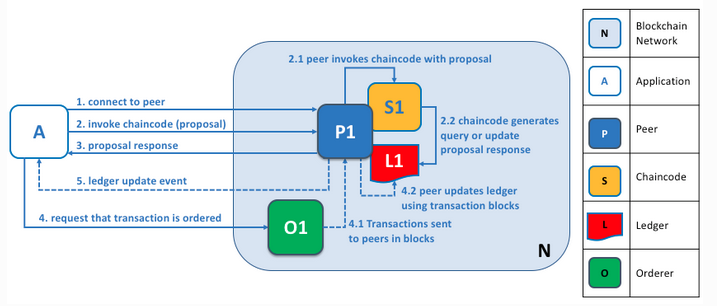
\includegraphics[width=1.0\linewidth]{Figures/Selection_171.png}}
    \caption{Flujos de consulta y actualización del \textit{ledger}. De \cite{hlf-peers}. }
    \label{fig:transaction_flow}
\end{figure}

Una actualización del \textit{ledger} requiere el consenso de una multitud de \textit{peers}, por lo cual se requieren más pasos:
\begin{enumerate}
    \item Cada \textit{chaincode} posee su propia política de aprobación que especifica cuantos \textit{peers}  tienen que aprobar la transacción para que ésta puede ser agregada al Blockchain. Cuando una aplicación quiere escribir datos o cambios, envía una propuesta a todos los \textit{peers}  necesarios para que la transacción pueda ser aprobada.
    \item Cada \textit{peer} determina que la propuesta sea válida, que la misma propuesta no se ha hecho anteriormente (protección contra un ataques de repetición) y que la aplicación tenga los permisos suficientes para realizar una escritura en el \textit{ledger}. Si se cumplen todas las condiciones, el \textit{chaincode} es ejecutado por todos los \textit{peers}  que lo recibieron y los resultados se envían en forma de una respuesta a la aplicación. Es importante entender que en el momento que la aplicación recibe las respuestas, todavía no se cambió el estado del Blockchain.
    \item La aplicación recibe las respuestas, verifica que todas sean iguales y si es el caso, manda su propuesta junto con las respuestas obtenidas al ``servicio para ordenar transacciones'' (\textit{ordering service}) para que la transacción sea agregada al \textit{ledger}.  
    \item Un \textit{peer} especial llamado \textit{orderer} cumple con la función de recibir diferentes transacciones, ordenarlas cronológicamente en bloques de datos y publicarlas en la red. 
    \item Una vez que se emitió el bloque nuevo a todos los \textit{peers}  suscritos al \textit{ledger} correspondiente, los \textit{peers}  verifican que la transacción en sí es válida y que se cumplió con la política de aprobación requerida. Luego, la transacción se declara como válida o inválida.
    \item Al completar el proceso descrito, la aplicación cliente es informada sobre la validez de la transacción y sobre su inclusión en el Blockchain. Debido al procesamiento requerido, la respuesta puede demorar varios segundos.
\end{enumerate} 

Vale aclarar que una ``actualización'' en este contexto no sobre escribe valores existentes: como en todas las implementaciones Blockchain, el \textit{ledger} es inmutable y no soporta operaciones de borrado o sobre escritura. ``Actualizar'' al Blockchain entonces significa simplemente agregar información nueva.

\section{Canales}
En la sección anterior, se explicó que un bloque nuevo es emitido a todos los \textit{peers}  suscritos a un \textit{ledger}. A continuación se va a explicar cómo funciona dicha subscripción. En Hyperldeger Fabric se usa un concepto llamado ``canales''.

Un canal describe un conjunto de \textit{peers}, un servicio de pedidos y un \textit{ledger} con su respectivo \textit{chaincode}. Todos los \textit{peers}, los nodos que se encargan del servicio de pedidos y las aplicaciones que se unen a un canal van a tener acceso a copias idénticas del mismo \textit{ledger}. Así, para que puedan existir varios \textit{ledgers} diferentes en una red, tienen que existir varios canales y los participantes que quieren acceder a los \textit{ledgers} en cuestión tienen que formar parte del canal correspondiente.

\begin{figure}[H] % Example image
\center{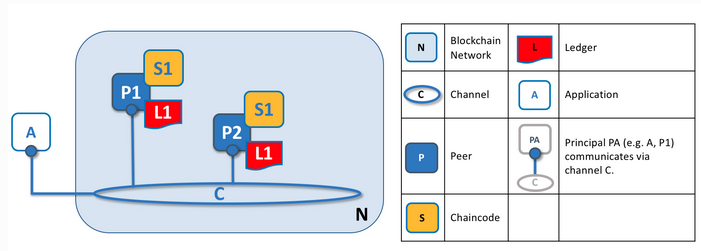
\includegraphics[width=1.0\linewidth]{Figures/Selection_172.png}}
\caption{Visualización del concepto de canal. De \cite{hlf-peers}.}
\label{fig:channels}
\end{figure}


\section{Agrupación de la red en organizaciones}

Tal como en Hyperledger Fabric se agrupan en canales los miembros de la red que acceden a un mismo \textit{ledger}, también se agrupan los \textit{peers}  según la organización a la que pertenecen.

El concepto de organización en Hyperledger Fabric describe una entidad que participa en la red y que conecta sus \textit{peers} a ella. La idea es que equivale a una organización en el mundo real: En el contexto del proyecto integrador, las organizaciones podrían ser las diferentes facultades que comparten información en una red Blockchain de la UNC.

Una organización puede aportar tantos \textit{peers}  a la red como desea. En la figura \ref{fig:organizations} la red está conformada por cuatro organizaciones y cada una tiene como mínimo un \textit{peer} conectado a un canal en común. También se puede observar que cada organización tiene su propia aplicación para acceder a los \textit{peers}: El desacoplado entre aplicación de usuario y \textit{chaincode} permite la implementación de una multitud de aplicaciones que consumen los datos compartidos de un mismo Blockchain.

\begin{figure}[H] % Example image
    \center{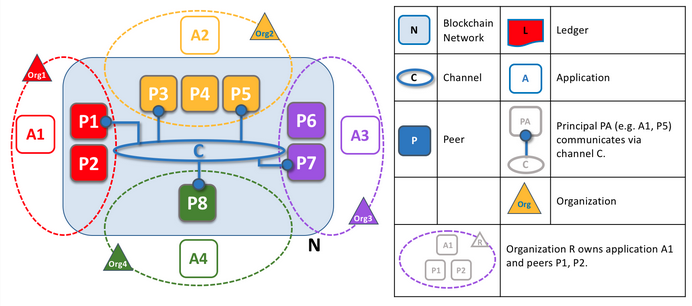
\includegraphics[width=1.0\linewidth]{Figures/Selection_173.png}}
    \caption{Una red Blockchain conformada por 4 organizaciones.}
    \label{fig:organizations}
\end{figure}

\section{La Identidad de los \textit{peers} en la red Blockchain}
\label{sec:identidad_de_peers}
¿Cómo reconoce la red qué \textit{peer} pertenece a qué organización? En Hyperledger Fabric, cada organización administra su propia Autoridad de Certificación (CA por sus siglas en inglés), que provee una identidad digital en forma de un certificado X.509 para cada \textit{peer} que se une a la red. La figura \ref{fig:identidad} describe un esquema de dos organizaciones con sus autoridades de certificación correspondientes.

Pero los certificados no solamente son para \textit{peers}: cualquier entidad que se quiere conectar a la red, también las aplicaciones, necesitan una identidad digital autorizada, sino su conexión será rechazada.

Si bien un \textit{peer} puede tener acceso a varios \textit{ledgers} compartidos entre diferentes organizaciones, siempre pertenece a una sola organización, la cual se determina con su identidad digital. Un \textit{peer} no puede ser compartido entre múltiples organizaciones.

\begin{figure}[H]
    \center{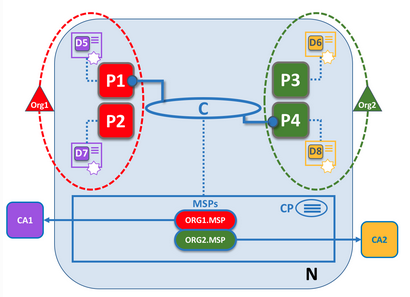
\includegraphics[width=0.7\linewidth]{Figures/Selection_176.png}}
    \caption{Una red compuesta de dos organizaciones, sus respectivas autoridades de certificación y sus MSP. Cada \textit{peer} tiene una identidad digital asociada, \textit{peer} P1 por ejemplo se identifica en el canal con la identidad D5. De \cite{hlf-peers}.}
    \label{fig:identidad}
\end{figure}

Los flujos de autenticación y autorización en Hyperledger Fabric son manejados por un \textit{Membership Service Provider} o MSP. Éste trabaja a dos niveles:
\begin{itemize}
    \item El \textit{Membership Service Provider} a nivel de canal identifica a qué organización pertenece cada \textit{
    peer} y controla que la participación y la administración del Blockchain solamente puede realizarse por los \textit{peers}  con los derechos correspondientes.
    \item El \textit{Membership Service Provider} a nivel local está funcionando adentro de cada \textit{peer}: Su objetivo es verificar los derechos de acceso de lectura y escritura de los clientes o aplicaciones que se conectan a él con el objetivo de invocar \textit{chaincode}. 
\end{itemize}

La comunicación entre los diferentes \textit{peers}  funciona a través de un protocolo \textit{gossip}, pero para que todos los participantes de un canal empiecen a compartir información, es necesario que cada miembro tenga conocimiento de los demás miembros de la red. Para el descubrimiento de \textit{peers}  en un canal se define un mínimo de un \textit{anchor peer} por canal: \textit{peers}  de todas las organizaciones notifican al \textit{anchor peer} sobre los miembros que pertenecen a su organización y reciben información sobre otros \textit{peers}  de otras organizaciones como respuesta. Luego de la etapa de descubrimiento, todos los \textit{peers}  del canal pueden comunicarse entre ellos y el \textit{anchor peer} solamente se va a volver a necesitar cuando se agreguen nodos a la red o se apagan. Se recomienda que cada organización tenga su conjunto de \textit{anchor peers} así se evita un único punto de fallos.

\section{Los \textit{Ledgers} y el \textit{World State}} \label{sec:ledger_and_world_state}
En la presente sección, se van a definir con mayor detalle los términos Blockchain y \textit{ledger} bajo el contexto de Hyperledger Fabric.

\textit{Ledger} es un término del inglés cuya traducción directa es ``libro contable''. Describe un registro que contiene el estado actual de un negocio junto con un historial de transacciones que llevaron a dicho estado.

En un \textit{ledger} se almacenan datos respecto a un cierto negocio. Los datos se pueden ver como objetos del negocio, aunque solamente son abstracciones de dichos objetos. En el caso de uso presentado, un objeto sería un acta de una facultad y el estado del acta puede cambiar de válido a inválido en el caso de ser revocado.

En Hyperledger Fabric, el registro histórico que lleva al estado actual es el Blockchain. Está estructurado como un registro secuencial de bloques interconectados, donde cada bloque contiene una secuencia de transacciones, cada transacción representa una consulta o actualización del estado de los objetos almacenados. La figura \ref{fig:bc_hlf} representa la estructura en forma gráfica: se puede observar que no existen diferencias fundamentales con otras implementaciones como Bitcoin.

\begin{figure}[H]
    \center{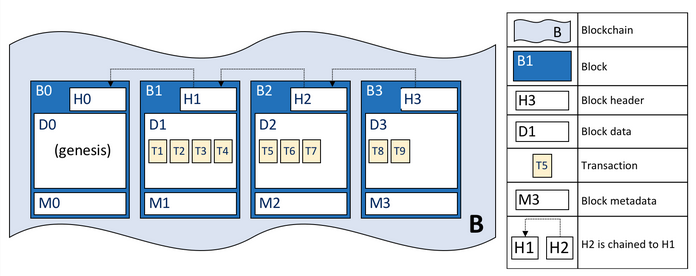
\includegraphics[width=0.8\linewidth]{Figures/Selection_186.png}}
    \caption{La estructura del Blockchain en Hyperledger Fabric. De \cite{hlf-ledger}.}
    \label{fig:bc_hlf}
\end{figure}

El Blockchain se almacena como un solo archivo y la operación más frecuente que se efectúa sobre éste es adjuntar bloques adicionales. Como el archivo no se encuentra indexado, consultas sobre el estado actual implican iterar de forma secuencial sobre los bloques almacenados, lo cual resulta ineficiente. Para resolver ese problema, Hyperledger Fabric extrae el estado actual del Blockchain y lo guarda en una base de datos. El conjunto de los estados actuales de todos los objetos lleva el nombre \textit{world state}.

Para el \textit{world state}, Hyperledger Fabric ofrece dos opciones de base de datos diferentes: La primera es LevelDB, un simple almacenamiento para datos en el formato clave-valor. Para almacenar objetos JSON con mayor complejidad, se recomienda CouchDB. Consultas en CouchDB se pueden hacer sobre claves y valores, no solamente sobre claves como en LevelDB. Además, CouchDB permite actualizar solamente partes del objeto JSON, mientras en LevelDB la actualización afecta al objeto entero.

\begin{figure}[H]
    \center{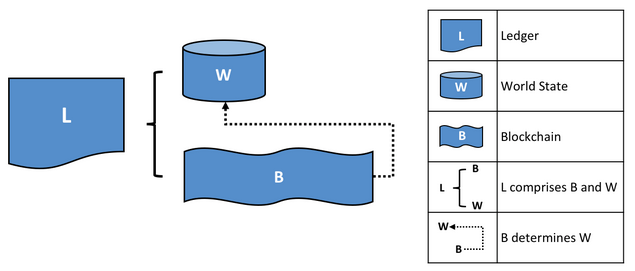
\includegraphics[width=0.8\linewidth]{Figures/Selection_185.png}}
    \caption{\textit{Ledger, World State} y Blockchain en contexto. De \cite{hlf-ledger}.}
    \label{fig:bc_ledger}
\end{figure}

En el contexto de Hyperledger Fabric, el conjunto de \textit{world state} y Blockchain reciben el nombre \textit{ledger}, como se ve en el gráfico \ref{fig:bc_ledger}. Al extraer el \textit{world state} del Blockchain y almacenarlo en una base de datos, se permite la indexación del estado actual y un alto rendimiento a la hora de realizar consultas.

\section{El servicio para ordenar transacciones}
\label{sec:ordering_service}
En el capítulo \ref{Chapter2} se explicó la importancia de un algoritmo de consenso y el funcionamiento de \textit{Proof of Work}, el algoritmo utilizado por una gran cantidad de implementaciones. Luego, junto con otras plataformas, se investigaron alternativas que surgieron con el objetivo de disminuir el consumo energético del algoritmo de consenso o de mejorar su rendimiento.

Los algoritmos de consenso, en su mayoría, tienen en común la ejecución de \textit{smart contracts}, la validación de transacciones y, la formación de bloques ejecutados por un mismo \textit{peer}. Esto significa un cuello de botella para el procesamiento de transacciones.

Hyperledger Fabric evita el problema descrito al distribuir ejecución, validación y formación de bloques entre diferentes participantes de la red: La ejecución del \textit{chaincode} se realiza en los \textit{peers} , la formación de bloques nuevos es realizada por \textit{peers}  especiales llamados \textit{orderer nodes} o nodos de ordenamiento y la validación es efectuada nuevamente por los \textit{peers} , una vez que el bloque nuevo se distribuyó en la red. 

Como los \textit{peers}, los \textit
{orderer nodes} pertenecen a una organización y obtienen sus credenciales criptográficas de una autoridad de certificación de dicha organización. Para la creación de un bloque nuevo, es posible establecer 2 criterios diferentes: 

\begin{enumerate}
    \item El primer criterio es el tiempo: Los \textit{orderer nodes} pueden ser configurados para generar un bloque nuevo cada intervalo de tiempo, siempre y cuando haya aunque sea una transacción esperando a ser procesada.
    \item El segundo criterio es el tamaño del bloque: Un bloque nuevo se agrega cuando se acumuló una cierta cantidad de transacciones que llena un bloque completo.
    \item Es posible combinar ambos criterios: Así, en momentos donde se efectúan pocas transacciones, se generan bloques más chicos cada cierto intervalo de tiempo y en momentos donde las cantidades de transacciones son altas, bloques nuevos son generados con mayor frecuencia y un tamaño máximo.
\end{enumerate}

Es posible modificar los parámetros mencionados cuando ya se generó un \textit{ledger}, para optimizar la performance de las escrituras.

Hyperledger Fabric provee tres servicios diferentes para la generación y el ordenamiento de bloques: con cualquiera de los tres, el Blockchain va a formarse de la misma forma, pero difieren en su trabajo de configuración y su funcionamiento interno.

\begin{itemize}
    \item \textbf{Solo: }Consiste de un solo \textit{peer} generador de bloques. No provee redundancia o protección a fallos. Su uso está pensado para tests o pruebas de conceptos.
    \item \textbf{Raft: }Un servicio de ordenamiento compuesto por un conjunto de \textit{orderer nodes} tolerante a fallos que implementa el protocolo Raft de la herramienta etcd.\cite{raft_algorithm}
    \item \textbf{Kafka: }Un servicio similar a Raft, tolerante a fallos, que utiliza Zookeeper para la gestión del \textit{cluster}. Su configuración y administración suelen ser más dificultosas que con Raft.
\end{itemize}


\section{Conclusión}
Las propiedades detalladas de Hyperledger Fabric reflejan las necesidades planteadas en el capítulo \ref{Chapter2} para una solución que consta de un Blockchain privado:

\begin{itemize}
    \item Los \textit{peers} y los \textit{ledgers} proveen el carácter distribuido también conocido de otras implementaciones.
    \item La posibilidad de la existencia de diferentes \textit{ledgers} permite mayor privacidad entre los participantes que si existiera un sólo \textit{ledger}. Su gestión es facilitada con canales.
    \item \textit{Peers} pertenecen a organizaciones y sus accesos se establecen a través de identidades digitales, lo cual facilita la administración de permisos de lectura y escritura.
    \item La división entre \textit{ledger} y \textit{world state} mejora el rendimiento de lecturas: el hecho de que el \textit{world state} se encuentra indexado, elimina la necesidad de iterar sobre los bloques del \textit{ledger} para consultar el último estado de la información.
\end{itemize}


